\documentclass[10pt,twocolumn,letterpaper]{article}

\usepackage{iccv}
\usepackage{times}
\usepackage{epsfig}
\usepackage{graphicx}
\usepackage{amsmath}
\usepackage{amssymb}

% Include other packages here, before hyperref.
\usepackage[labelfont=bf, skip=3pt]{caption}
\captionsetup{labelsep=period}
\usepackage{footmisc}

% If you comment hyperref and then uncomment it, you should delete
% egpaper.aux before re-running latex.  (Or just hit 'q' on the first latex
% run, let it finish, and you should be clear).
\usepackage[pagebackref=true,breaklinks=true,letterpaper=true,colorlinks,bookmarks=false]{hyperref}

% \iccvfinalcopy % *** Uncomment this line for the final submission

\def\iccvPaperID{****} % *** Enter the ICCV Paper ID here
\def\httilde{\mbox{\tt\raisebox{-.5ex}{\symbol{126}}}}

% Pages are numbered in submission mode, and unnumbered in camera-ready
\ificcvfinal\pagestyle{empty}\fi
\begin{document}

%%%%%%%%% TITLE
\title{What Makes Deep Network Representations Good for Visual Recognition?}

\author{First Author\\
Institution1\\
Institution1 address\\
{\tt\small firstauthor@i1.org}
% For a paper whose authors are all at the same institution,
% omit the following lines up until the closing ``}''.
% Additional authors and addresses can be added with ``\and'',
% just like the second author.
% To save space, use either the email address or home page, not both
\and
Second Author\\
Institution2\\
First line of institution2 address\\
{\tt\small secondauthor@i2.org}
}

\maketitle
%\thispagestyle{empty}

\begin{abstract}

Representations of artificial neurons in deep neural networks have been demonstrated to be highly effective and robust for various visual recognition tasks~\cite{krizhevsky2012imagenet, sermanet2013overfeat, donahue2014decaf}.
Nevertheless, our understanding of them arguably remains limited.
In this paper, we address two important and practical questions: (1) why deep networks are better than shallow networks, and (2) among networks of the same depth, why certain networks are better than the others. Using methods which support characterizing both first-order and second-order properties of scalar and vector representations, we considered the case study of face pair matching and conducted a large-scale experiment. This experiment examined 200 randomly generated shallow and deep networks, with the results analyzed through a series of measures designed to quantify the differences in representations. 
We conclude through this principled analysis that deep representations are quantitatively better than shallow representations, and overall 71\% of the variance in the performance of deep networks can be explained with our measures, both of which are confirmed using statistical tests for the first time.

%(\ie optimal stimulus) (\ie invariance and selectivity paths)
%use X as example of deep networks
%concern about deep networks; how alleviated via this work

\end{abstract}

\section{Introduction}

\begin{figure}
\begin{center}
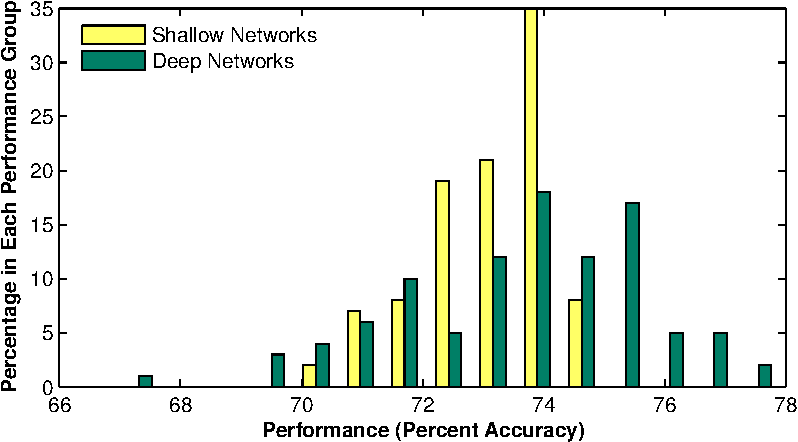
\includegraphics[width=0.90\columnwidth]{Figs/e_fig7s_compact-crop.pdf} 
\end{center}
\caption{{\bf What makes a deep network good?}
In existing work, researchers have mostly tried to produce one ``best'' network architecture (\ie a hyperparameter set, either through manual tuning or automated hyperparameter search), which is subsequently evaluated on a particular benchmark. However, as exemplified in this figure, when considering a larger population of networks \cite{cox2011beyond}, it is not fully clear to us why in practice deep networks (\eg two or more levels) outperform shallow networks (\eg one-level), and why certain networks are better than the others, given their broad distribution of performance on a task like face pair matching for the LFW-a data set (shown above)~\cite{LFWTech, wolf2011effective}.
%However, it is not fully clear that in practice (1) why deep networks are better than shallow networks, and (2) among networks of the same depth, why certain networks are better than the others.
%As exemplified in the figure, deep (\ie two-level) networks not only on average outperform shallow (\ie one-level) networks \cite{cox2011beyond}, but also exhibit a wide range of performance differences on LFW-a face recognition \cite{LFWTech, wolf2011effective}.
} % (\eg optimal stimulus). %and (sometimes) characterized its properties
\label{fig:perf}
\end{figure}

Although deep neural networks have been successfully pushing the boundaries of computer vision by breaking the records of ImageNet Challenges (ILSVRC) year after year~\cite{krizhevsky2012imagenet, sermanet2013overfeat, szegedy2014going}, our understanding of the properties of these networks arguably remains limited, since we cannot yet fully answer the question ``what makes a deep network good?'' In this paper, we investigate two important facets of this question: (1) why deep networks are better than shallow networks, and (2) among networks of the same depth, why certain networks are better than others (Fig.~\ref{fig:perf}). Specifically, from the point of view that successful networks are forming ``better'' representations of visual inputs that are more separable to the final-stage linear classifiers, we want to identify the crucial properties that are required for forming (or learning) better representations.

%which can be potentially useful in improve representation learning 

%\newcommand{\ivec}{\mathrm{vec}^{-1}}
%$f({\bf{x}}) = \left\| {\bf{K}} \otimes \ivec\left({\bf{x}}\right) \right\|_{F}$
\newcommand{\expstimdim}{For simplicity, a stimulus being 2-dimensional (\ie ${\bf{x}} \in \mathbb{R}^{\sqrt{N} \times \sqrt{N}}$) or vectorized (\ie ${\bf{x}} \in \mathbb{R}^N$) are used interchangeably.}

%first order, second order, flexibility
{\bf Existing work.} 
Given an artificial neural network $f$, the study of how $f$ represents a high dimensional stimulus\footnote{\expstimdim} ${\bf{x}} \in \mathbb{R}^N$ as a representation 
${\bf{r}} = f\left( {\bf{x}} \right)$ in existing work mainly focused on the first-order (\ie linear) characterization of $f$---the analysis of optimal stimuli, stimuli which lead to the strongest responses of given neurons.
For single-level convolutional networks using squared pooling, \ie $f({\bf{x}}) = \left\| {\bf{K}} \otimes {\bf{x}} \right\|_{F}$, the optimal stimulus was shown to be analytically approximable \cite{saxe2011random} using a Gabor-like filter, whether the convolution kernel $\bf{K}$ is structural or random.
For multi-level convolutional networks, the optimal stimuli of neurons from various depths were numerically approximated \cite{ngiam2010tiled, le2012building, zeiler2014visualizing, simonyan2013deep} to qualitatively show neurons in deeper layers are tuned to more complex visual patterns.
The generalized concept of optimal stimulus in considering groups of neurons can also be adopted to study the representations by inverting them \cite{mahendran2014understanding}.

In addition to the first-order characterization, the analysis of invariance and selectivity properties of neurons (\eg changes in stimuli which given neurons are least and most sensitive to, how small or large the changes are, \etc) was adopted in a few works. This can be viewed as the second-order characterization of $f$, and parametric deformation in stimuli was the most commonly used setup.
For example, translation, rotation, scaling, \etc of the stimulus were used in~\cite{goodfellow2009measuring, zeiler2014visualizing} to test the invariance and selectivity of neurons.
Similar deformations were also adopted in \cite{lenc2014understanding}, but extended to analyze more advanced properties (\ie equivariance and equivalence) of groups of neurons.
More generalized setups that, \eg, utilize local quadratic information (\ie the Hessian) or ``global'' numerical searches in the stimulus space, even though they do exist, are less explored in the context of artificial neural network studies.
For quadratic networks, \ie $f\left({\bf{x}}\right) = \frac{1}{2}{\bf{x}}^{T}{\bf{Qx}}+{\bf{L}}^{T}{\bf{x}}+c$, through eigendecomposing the quadratic term $\bf{Q}$ (\ie the Hessian), local invariance and selectivity directions can be analytically derived \cite{berkes2006analysis}, which correspond to eigenvectors of the least and most negative eigenvalues.
This method was also generalized onto multi-layer convolutional networks by numerically estimating the Hessian \cite{ngiam2010tiled}.
For multi-layer networks, characterization of the ``global'' invariance of single neurons can also be achieved by numerically searching for non-local (\ie farther to the optimal stimuli) solutions \cite{erhan2010understanding}.

%with its frequency component collocated with the peak of the Fourier spectrum of convolution kernel $\bf{K}$
%(\ie farther to the optimal stimuli)

%{\bf Contributions of this work.} Comparatively, the characterization of representations in this work is designed to be general and unbiased such that both first- and second-order methods can be supported for single neurons or groups of neurons, without assuming any \emph{de facto} property in the solutions (\eg parametric deformations as used for studying invariance in previous works).
%Additionally, with the strong statistical significance of results obtained from the large-scale experiments on 100 shallow and 100 deep networks, totally 6,400 artificial neurons, we argue that our observations toward answering the differences between (shallow \vs deep) and among (deep) representations are highly evident and comprehensive, which cab be summarized as ***

\section{Representation Characterization}

\begin{figure}
\begin{center}
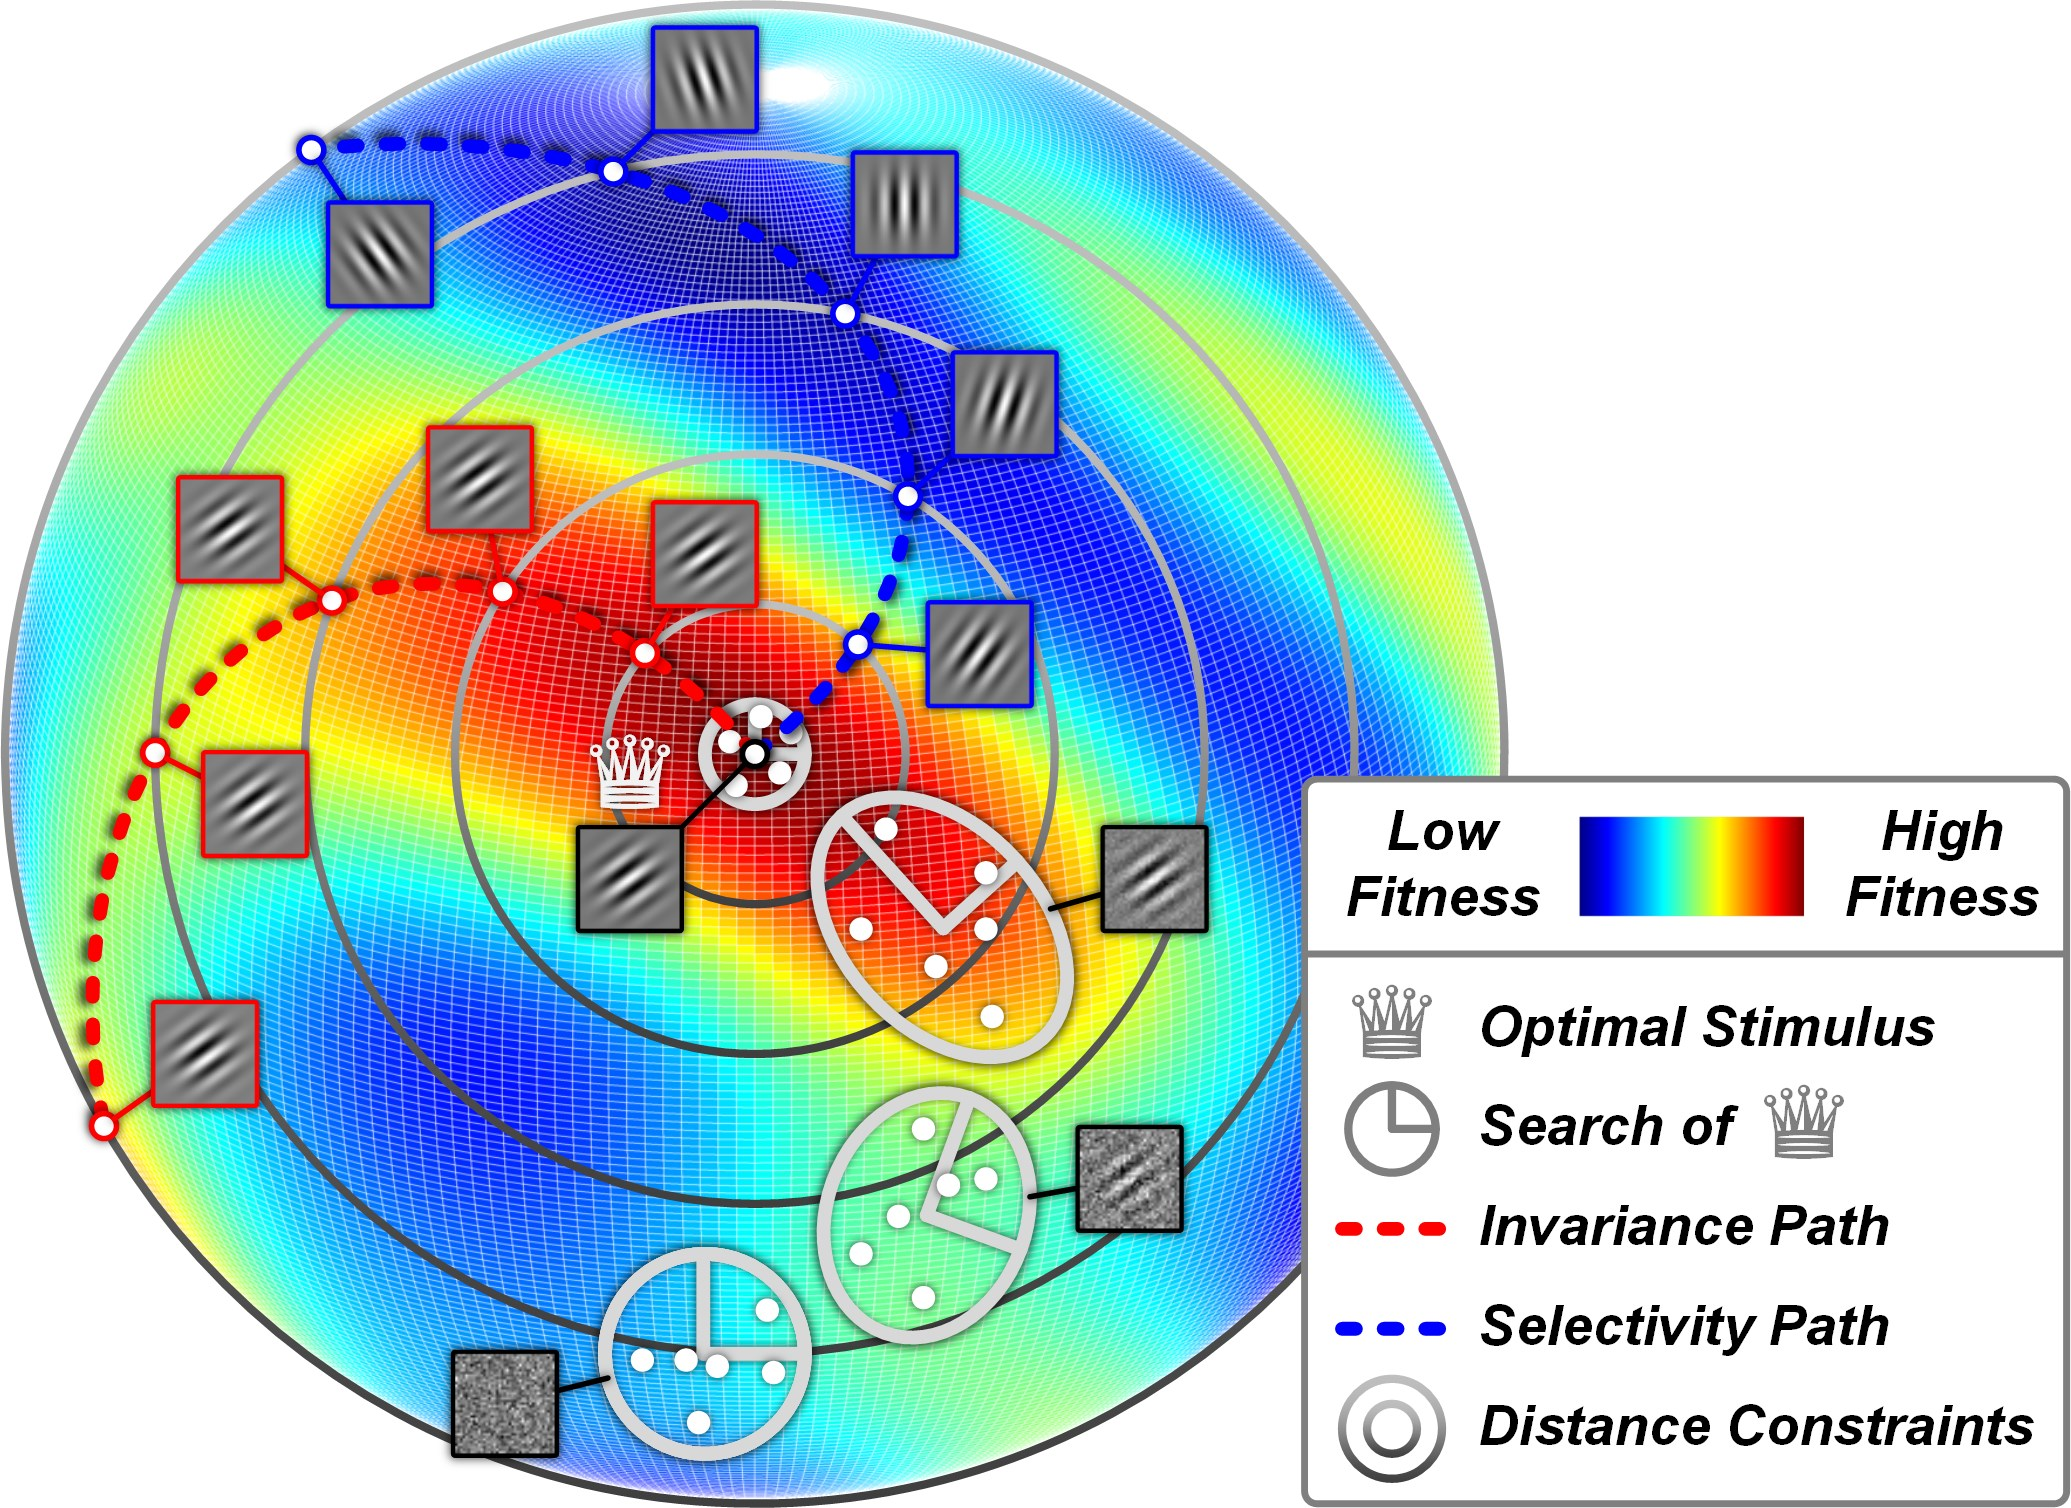
\includegraphics[width=1.0\columnwidth]{Figs/methods.jpg} 
\end{center}
\caption{{\bf Representation characterization methods.}
On the spherical (\ie constant energy) constraint of the $N$ dimensional stimulus space, similar to previous work, the first-order property (\ie optimal stimulus $\hat{\bf{x}}$) of a representation $\bf{r}$ is first iteratively searched (as the evolution of light gray eclipses) and analyzed.
However, unlike most previous work, the second-order properties (\ie invariant path $\lbrace \bf{x}^{+}_{\delta} \rbrace$ and selectivity path $\lbrace \bf{x}^{-}_{\delta} \rbrace$) at distances $0.1\pi$ to $0.5\pi$ from the optimal stimulus are also searched and analyzed.
Additionally, these methods are capable of characterizing both scalar and vector representations, where the ``fitnesses'' to be optimized correspond to Eq.~\ref{eq:O1}, \ref{eq:I1}, \ref{eq:S1} and Eq.~\ref{eq:O2}, \ref{eq:I2}, \ref{eq:S2}, respectively.
In this example, the scalar representation (\ie response) of the given neuron is tuned to a $45^{\circ}$ Gabor filter and invariant to phase changes, but selective to orientation changes.
}
\label{fig:methods}
\end{figure}

% DEFINE X & f????
%representational property 

To study the representations inside an artificial neural network, methods adopted in this work include: (1) first-order (\ie linear) characterization, or search and analysis of optimal stimuli, and (2) second-order (\ie quadratic) characterization, or search and analysis of invariance and selectivity paths (\ie eigenvectors of the largest and smallest eigenvalues), which are generalized and improved from previous work.
$\bf{r}$ is defined as a scalar representation (\ie $\bf{r} \in \mathbb{R}$) when considering single neurons and a vector representation (\ie ${\bf{r}} \in \mathbb{R}^C$) when considering groups of neurons (with group size $C$).
Our methods support characterizing both scalar (using Eq.~\ref{eq:O1}, \ref{eq:I1}, \ref{eq:S1}, though Eq.~\ref{eq:O2}, \ref{eq:I2}, \ref{eq:S2} can be used as well) and vector (using Eq.~\ref{eq:O2}, \ref{eq:I2}, \ref{eq:S2}) representations in a unified way.
The search phases defined via these equations will be introduced in the following subsections, and the analyses of search results using representation measures will be covered in Sec.~\ref{sec:exp}.

% SEARCH HERE, ANALTSIS MEASURES LATER
%$\bf{r}$, in this work, is equivalent to the response(s) of artificial neuron(s), and
%Arguably, for studying neural networks, especially when regarding task-related (\eg recognition) performances, the importance of characterizing vector representations can be greater than of characterizing scalar representations, considering the differences in representational powers. 

While no specific knowledge of the network itself is assumed, we do restrict the space of stimuli considered with a constant energy constraint $\left\| \bf{x} \right\| = E$, where $E$ is set to $1$ in all mathematical derivations for simplicity, but set to the average energy of task-related images in our experiments.
Since neurons can often be modulated by stimulus contrasts, which is less interesting when considering pattern selectivities, limiting the stimulus space in this manner effectively avoids degenerate solutions that simply maximize stimulus contrasts, and reduces the range of possible stimuli to consider.

%, the setting of $E=1$ is used for the rest of the paper, while  $E$ {was} set 
%, based on prior knowledge of (artificial) neuronal response properties.

\subsection{First-Order Property Characterization}

In this work, the optimal stimulus is defined and numerically derived as 
\begin{align}
\hat{\bf{x}} &= \underset{\bf{x}} {\arg\max} f\left(\bf{x}\right) \label{eq:O1} \\
&= \underset{\bf{x}}{\arg\max} \left( e^{-\left\|f\left(\bf{x}\right)-f\left(\tilde{\bf{x}}\right)\right\|} \right); \label{eq:O2}
\end{align}
subject to the spherical constraint $\left\| \bf{x} \right\| = 1$. 
As visualized in Fig.~\ref{fig:methods}, this process involves an iterative search on the non-convex fitness landscape, which in fact can be handled efficiently by most of the modern numerical solvers, especially when analytical derivatives (\ie backpropagation gradients) are available.
In this work, we adopted the CMA-ES solver \cite{hansen2001completely}, which does not rely on analytical gradients and instead stochastically estimates numerical derivatives (\ie inverse Hessian), and worked reasonably well in our experiments.
When considering a vector representation (using Eq.~\ref{eq:O2}), this process is equivalent to optimizing the response of an ``imaginary neuron'' tuned to a reference stimulus $\tilde{\bf{x}}$.

% $\exp\left( -\left\|f\left(\bf{x}\right)-f\left(\tilde{\bf{x}}\right)\right\| \right)$
%Or equivalently, optimal stimulus of an imaginary neuron tuned to the 

\subsection{Second-Order Property Characterization}

\newcommand{\expdiff}{The way the simple linear constraint is constructed to enforce the exploration of a larger extent of the fitness landscape is also one of the main differences compared to \cite{erhan2010understanding}.}

With respect to the optimal stimulus $\hat{\bf{x}}$, the searches of invariance and selectivity paths, which consist of sets of invariant stimuli $\left\lbrace \bf{x}^{+}_{\delta} \right\rbrace$ and selective stimuli $\left\lbrace \bf{x}^{-}_{\delta} \right\rbrace$ respectively, are formulated as
\begin{align}
\bf{x}^{+}_{\delta} &= \underset{\bf{x}_{\delta}}{\arg\max} f\left(\bf{x}_{\delta}\right) \label{eq:I1} \\
&= \underset{\bf{x}_{\delta}}{\arg\max} \left( e^{-\left\|f\left(\bf{x}_{\delta}\right)-f\left(\hat{\bf{x}}\right)\right\|} \right); \label{eq:I2} \\
\bf{x}^{-}_{\delta} &= \underset{\bf{x}_{\delta}}{\arg\min} f\left(\bf{x}_{\delta}\right) \label{eq:S1} \\
&= \underset{\bf{x}_{\delta}}{\arg\min} \left( e^{-\left\|f\left(\bf{x}_{\delta}\right)-f\left(\hat{\bf{x}}\right)\right\|} \right); \label{eq:S2}
\end{align}
in which $0 < \delta \le \frac{\pi}{2}$, subject to $\left\| \bf{x}_{\delta} \right\| = 1$ and $\langle \bf{x}_{\delta} , \hat{\bf{x}} \rangle = \cos\left(\delta\right)$. 
As visualized in Fig.~\ref{fig:methods}, the invariance path characterizes the $N$ dimensional curve that leads toward (or ideally, maintains at) a fitness as high as possible while moving away from the optimal stimulus, and the selectivity path characterizes the curve that leads toward fitness as low as possible while moving away.
The search process is implemented as multiple runs of maximization and minimization on discretized $\delta \in \left\lbrace 0.1\pi, 0.2\pi, 0.3\pi, 0.4\pi, 0.5\pi\right\rbrace$ as the circular distance constraints shown in Fig.~\ref{fig:methods}, where each run is initialized with the result from the previous run (and the $0.1\pi$ run directly with optimal stimulus $\hat{\bf{x}}$) to increase the path continuity and searching speed\footnote{\expdiff}.
In this work, the distance constraint $\delta$ only goes up to $\frac{\pi}{2}$, since on the $N$ dimensional sphere, stimuli that fall in $\frac{\pi}{2} < \delta \le \pi$ are simply ``negatives'' of those in $0 < \delta \le \frac{\pi}{2}$, which are of less uniqueness and interest in general. 
The same process can also be performed with respect to a reference stimulus $\tilde{\bf{x}}$, especially for vector representations, where the invariance and selectivity of the ``imaginary neuron'' are again characterized equivalently.

%; nevertheless, going up to the full range $0 < \delta \le \pi$ is numerically straightforward.

\section{Experiments}
\label{sec:exp}
%\subsection{Experimental Setup}
% \cite{fukushima1980neocognitron, lecun1998gradient, riesenhuber1999hierarchical, krizhevsky2012imagenet}

For our experiments, a simplified variety of deep convolutional neural networks---the Spatio-Temporal Hierarchical Object Representation (STHOR) model \cite{pinto2009high, sthor}---{was} adopted.
Like other deep networks, it consists of the standard cascade of convolution, nonlinear activation, pooling layers, \etc (which together define a single ``level'' in this work). However, its convolution kernel weights are  randomly assigned rather than trained.
Though not matching the performances of deep networks trained on massive quantities of data \cite{krizhevsky2012imagenet}, it can in fact be surprisingly competitive for a variety of tasks, especially in the regime where large quantities of training samples are not readily available \cite{pinto2009high, cox2011beyond, viglarge}.
Most importantly, since it does not require training (except for the linear SVM on top of the representations extracted), a large number of networks with diverse hyperparameters can be rapidly generated and compared, which is particularly useful in this study where relative, instead of absolute task performances, are of primary interest. 
As one might be concerned that comparing randomly weighted networks will not tell much about representations, since they might as well be random, our results will suggest otherwise.

\newcommand{\expsettings}{\Ie 32 channels of filters in the top level's convolution layers, a simple setting with reasonable performance.
Following the terminology in recent work, shallow and deep neurons corresponded to \texttt{pool1} and \texttt{pool2} layers respectively.
Stimulus dimensionalities of the shallow and deep neurons {were} $N=121$ and $441$ (\ie spatially overlapping $11\times11$ and $21\times21$ receptive fields). % respectively
Other minor changes included: nonlinear activations all simplified to \emph{ReLU} \cite{krizhevsky2012imagenet} mode and normalizations all in subtractive mode.
Overall, the architectures were more similar to those in \cite{simonyan2014very}, except pooling operations can be \emph{average}, \emph{squared}, or \emph{max-like} in our case.
}

\newcommand{\exptask}{We chose face images over object images for our recognition task because facial patches can be easily aligned and compared against our results. However, our methods and measures are not limited to just face images.}

In the experiments, 100 shallow (\ie one-level) networks and 100 deep (\ie two-level) networks {were} randomly generated (though all have 32 top-layer neurons\footnote{\expsettings}) and tested to see how their representations differ with networks' depths and affect networks' performances on face pair matching\footnote{\exptask} tasks against the LFW-a dataset \cite{LFWTech, wolf2011effective} as shown in Fig.~\ref{fig:perf}. %, using 10-fold cross validation on view 2.
The fitness landscapes of shallow and deep representations in our case are both non-convex, therefore there is no guarantee that optimality can be achieved through any optimization method.
However, by carefully adjusting the numerical solver and monitoring the quality of solutions, we argue that informative local optima can still be discovered and used to characterize the representations.
Specifically, all numerical optimizations {were} executed multiple times from different random initial stimuli, for increasing quality of the numerical solutions (of optimal stimuli and invariance and selectivity paths, with 2 runs executed and the better kept), and at the same time, for providing statistical samplings of the solution spaces (of encoding specificities and invariance and selectivity subspace properties, as detailed later).

% (as shown in Fig.~\ref{fig:perf})
%---accuracy of identifying pairs of different pictures from the same person and rejecting those from different persons---

\subsection{Results: Shallow \textbf{\textit{vs.}}~Deep Representations}

\begin{figure*}
\begin{center}
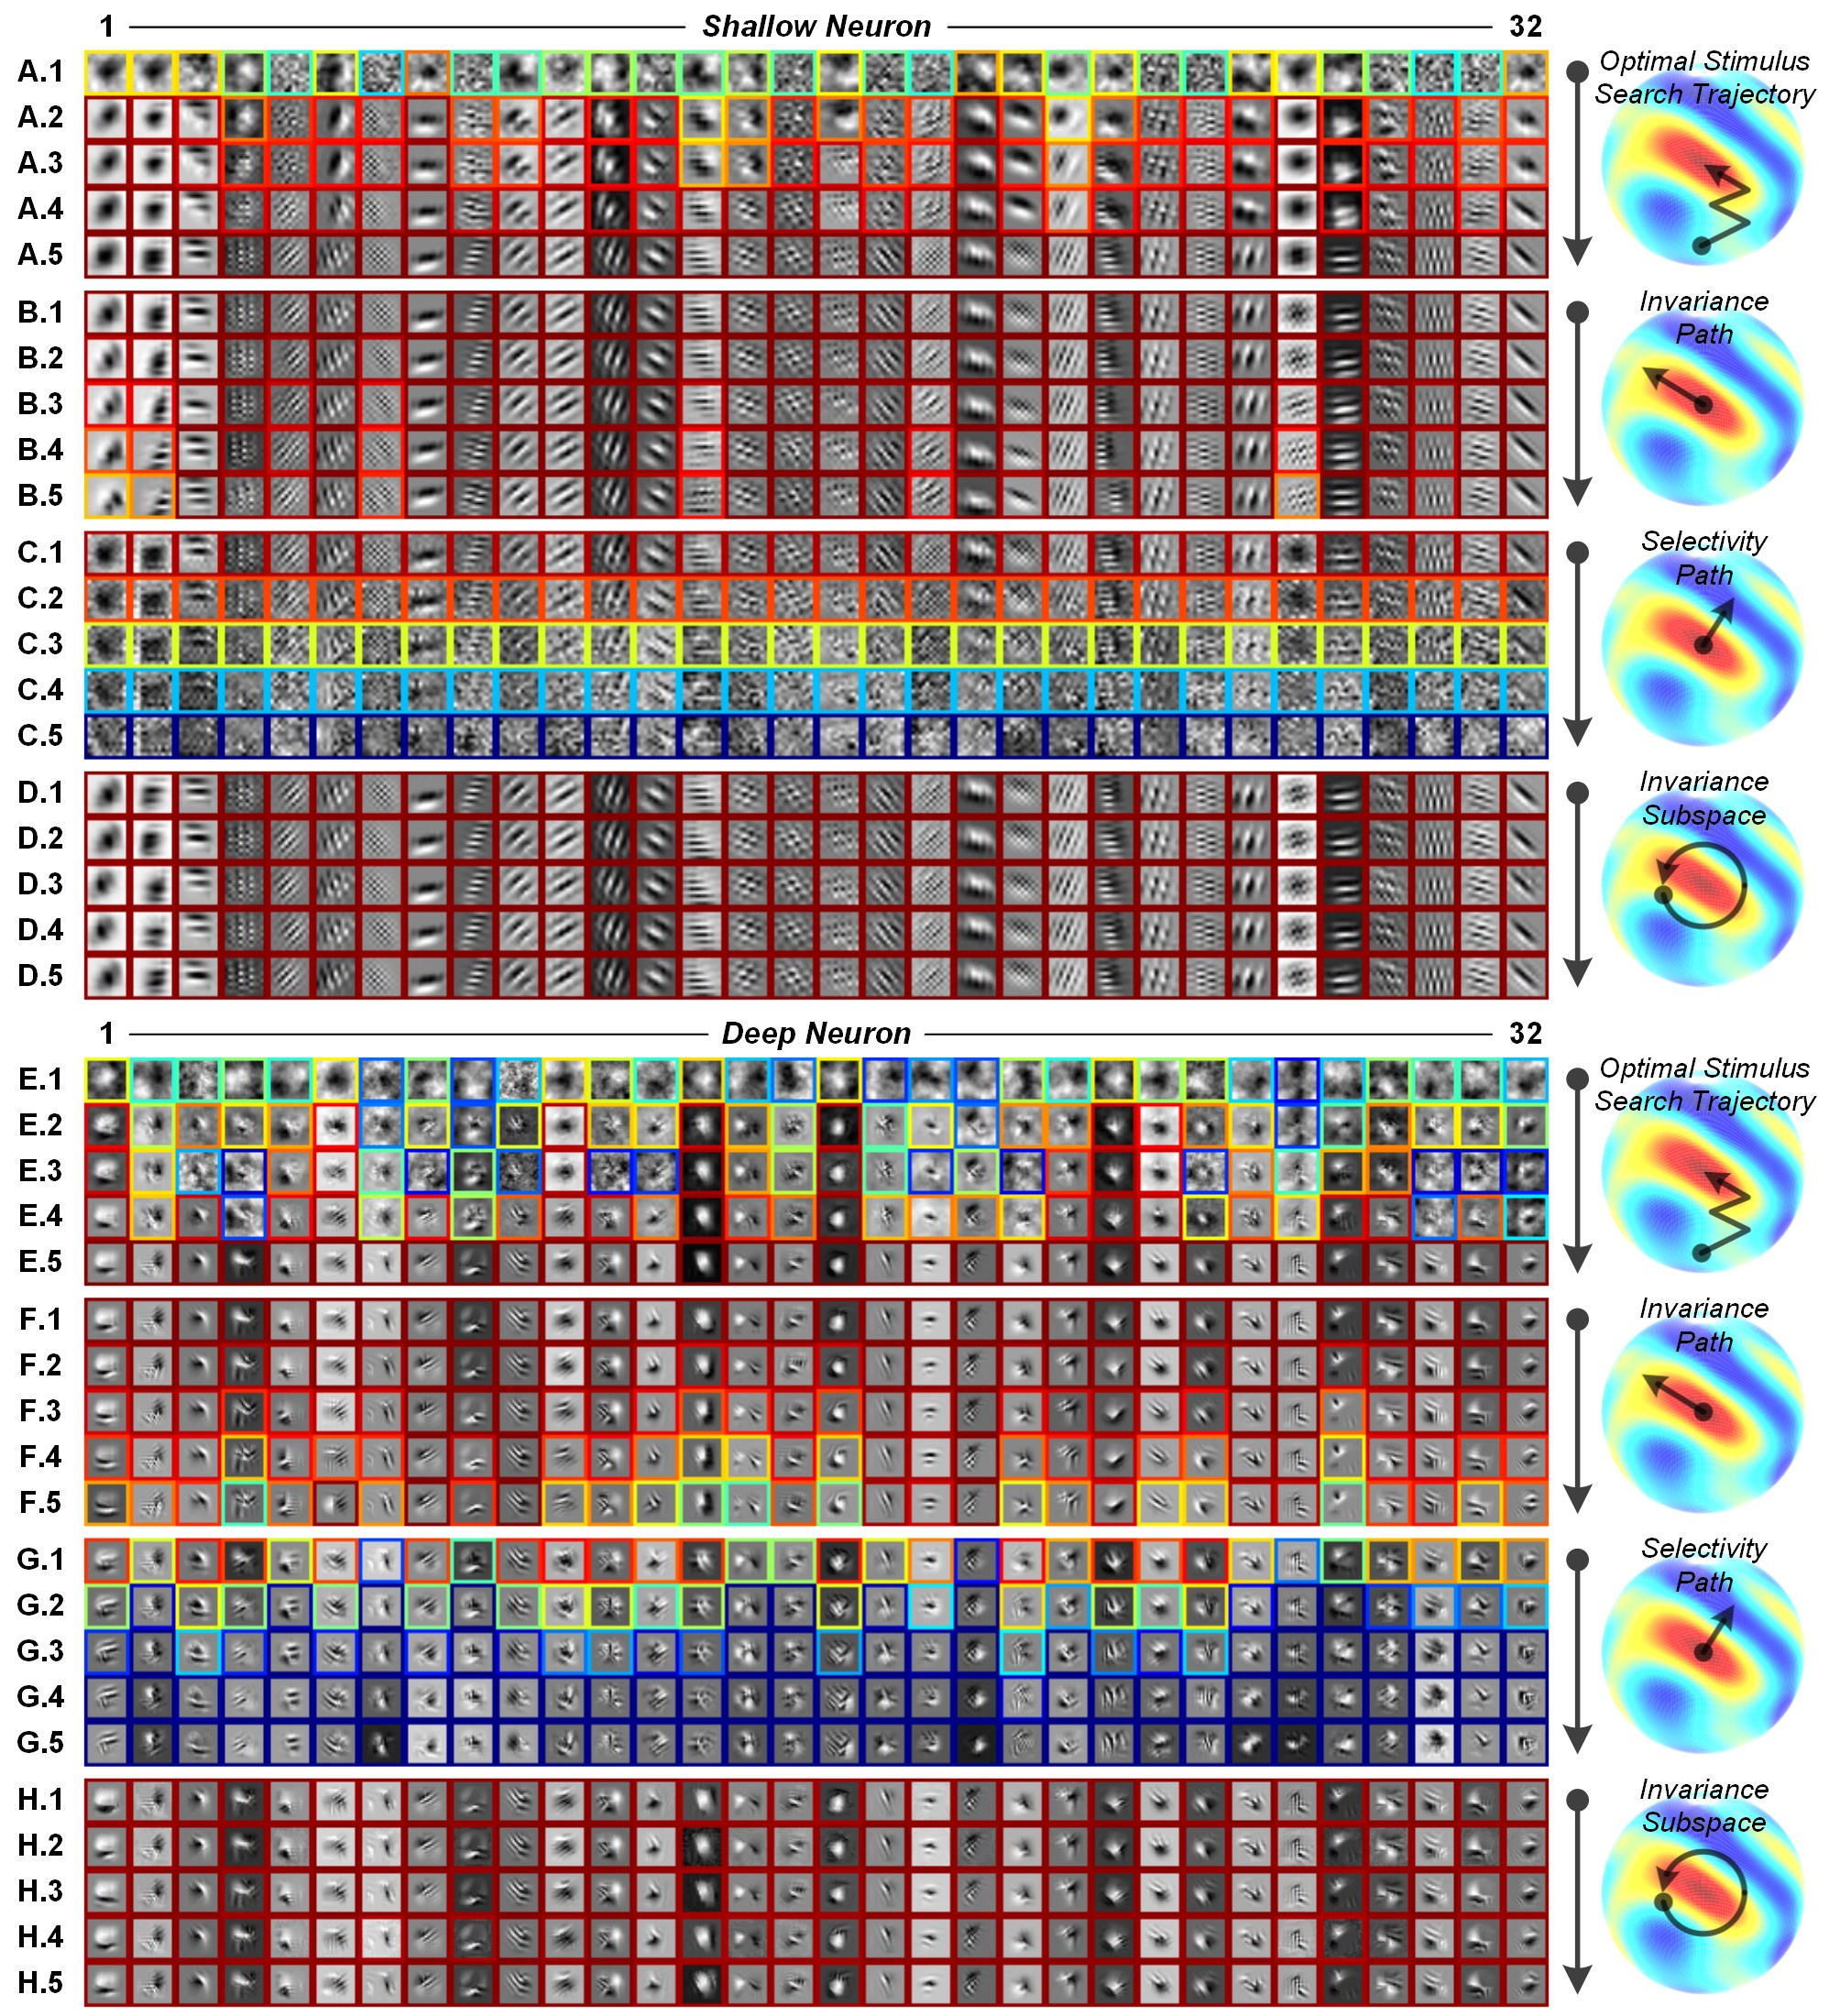
\includegraphics[width=0.80\textwidth]{Figs/pic1.jpg} 
\end{center}
\caption{{\bf Visualization of properties of shallow (A--D) and deep scalar representations (E--H).}
Color of the boarder of an image indicates the fitness of the representation (\ie response of the neuron) driven by the image, with color map following the definition in Fig.~\ref{fig:methods}.
A and E show the search trajectories of \emph{optimal stimuli} of all 32 neurons from the best performing shallow and best performing deep networks, respectively, where A.1 and E.1 show the initial $1/f$ random stimuli, A.5 and E.5 the resultant optimal stimuli, and A.2--4 and E.2--4 three intermediate steps corresponding to the three largest curvatures in the fitness histories.
B and F show the \emph{invariance paths} of shallow and deep neurons, starting from the corresponding optimal stimuli show in A.5 and E.5, moving from $0.1\pi$ (B.1 and F.1) to $0.5\pi$ (B.5 and F.5) away accordingly.
C and G show the \emph{selectivity paths} of shallow and deep neurons, with definitions following B and F.
D and H show the \emph{invariance subspaces} sampled $0.1\pi$ away from the optimal stimuli, with 5 out of 20 results randomly selected.
Comparatively, \emph{deep neurons show more complex and diverse representational properties} than shallow neurons do.
} % do visually
\label{fig:allrep}
\end{figure*}

\begin{figure}
\begin{center}
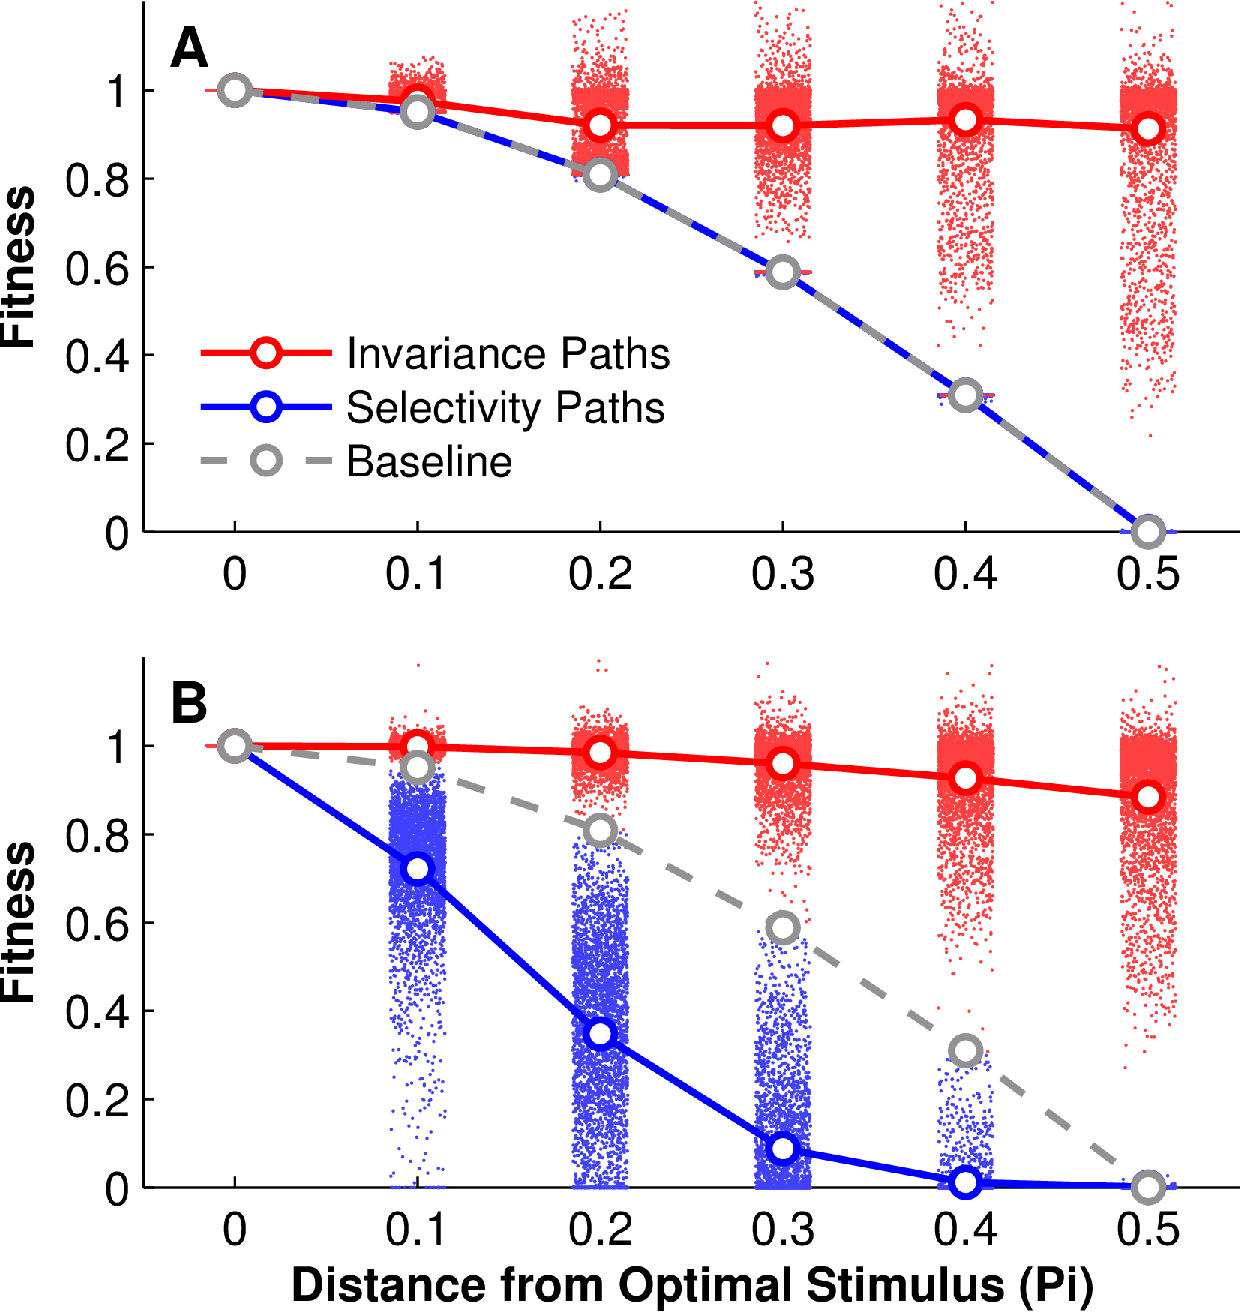
\includegraphics[width=0.75\columnwidth]{Figs/fig4.pdf} 
\end{center}
\caption{{\bf Fitness-distance analyses of shallow (A) and deep scalar representations (B).}
Fitnesses of invariance (red dots, \ie $\left\lbrace f\left(\bf{x}^{+}_{\delta}\right) \right\rbrace$) and selectivity paths (blue dots, \ie $\left\lbrace f\left(\bf{x}^{-}_{\delta}\right) \right\rbrace$) of all 3,200 shallow and 3,200 deep neurons are shown for comparison\protect\footnotemark.
Although both types of neurons show invariance, shallow neurons do not posses selectivity, since their selectivity paths overlap with the zero-selectivity baseline.
In other words, \emph{only deep neurons are selective}.
} %, and random walks (green dots, \ie $\left\lbrace f\left({\bf{x}}^{R}_{\delta}\right) \right\rbrace$)
%the dashed line, 
\label{fig:fda}
\end{figure}

\begin{figure}
\begin{center}
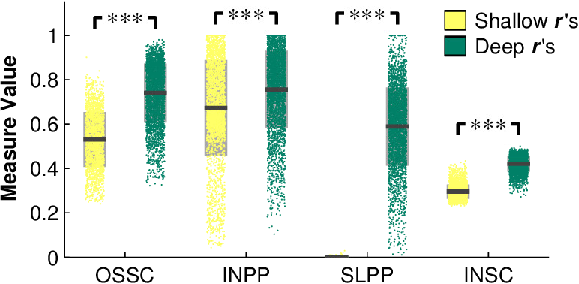
\includegraphics[width=0.80\columnwidth]{Figs/fig5.pdf} 
\end{center}
\caption{{\bf Comparison of shallow and deep scalar representation measures.}
Representation measures from left to right are, optimal stimulus spectral complexity (OSSC), invariance path potential (INPP), selectivity path potential (SLPP), and invariance subspace capacity (INSC).
Sensitivity indexes ($d'$) between distributions are $1.63$, $0.42$, $4.73$, and $3.67$, and differences between means of distributions are all significant (***), which suggest \emph{deep representations are quantitatively and significantly better than shallow representations}.
} %, in which data points from shallow networks (left distributions) and deep networks (right distributions) are shown side by side
\label{fig:pair}
\end{figure}

{\bf Optimal stimulus spectral complexity.} Figure \ref{fig:allrep}A and \ref{fig:allrep}E illustrate the trajectories of optimal stimulus searches of 32 top-layer neurons from the best performing shallow network and 32 from the best performing deep network respectively.
To further increase the searching speed, the initial stimulus {was} selected from 1000 ${1}/{f^{\alpha}}$ random stimuli with the best fitness, where $\alpha \in \left\lbrace -4,-3,-2,-1,0 \right\rbrace$, without overly sacrificing the nature of random initialization.
From the results, first, the response landscapes of deep neurons are noticeably more complex than those of shallow neurons, as a large fraction of searching trajectories for deep neurons actually go down then up before reaching the (local) optima, which also suggests the numerical solver can handle non-convexity reasonably well.
Second, the optimal stimuli of deep neurons are also relatively more complex (\ie consisting of more textural components) than those of shallow neurons (which are more uni-textured or Gabor-like).
To quantify such differences, the spectral complexity measure, which is estimated through the $L^{1}$ norm of the (2 dimensional) Fourier power spectrum of optimal stimulus, \ie $\left\| \mathcal{F}(\hat{\bf{x}}) \right\|_{1}$, is adopted, where a higher value suggests higher non-sparsity (\ie more spectral components required to represent the visual stimuli).

\footnotetext{A small fraction of invariance paths in fact have fitnesses higher than the optimal stimuli's due to a non-convex problem's nature, which however does not cause noticeable differences in the resultant statistics.}

\newcommand{\defbaseline}{Given a single inner-product neuron $f({\bf{x}}) = {\bf{w}}^{T}{\bf{x}}$ and $\left\| \bf{x} \right\| = 1$, we have $\hat{\bf{x}} = \bf{w}$ and thus $f({\bf{x}}_{\delta}) = {\hat{\bf{x}}}^{T}{\bf{x}}_{\delta} = \cos(\delta)$ by definition.}

{\bf Invariance and selectivity path potential.} Figure \ref{fig:allrep}B/C and \ref{fig:allrep}F/G illustrate the invariance and selectivity paths on the same sets of shallow and deep neurons as in \ref{fig:allrep}A and \ref{fig:allrep}D.
While invariance paths are mostly phase changes and selectivity paths are leading toward meaningless noises (all at the same falloff rate) for shallow neurons, both types of paths consist of sophisticated shape deformations for deep neurons.
As further demonstrated in the fitness-distance diagrams \cite{jones1995fitness} (Fig.~\ref{fig:fda}), on average, although shallow neurons have good invariance (\ie red curve stays high), they do not have any selectivity (\ie blue curve drops slow), while deep neurons show both good invariance and selectivity (\ie red curve stays high and blue curve drops fast).
For scalar representations, we can define the invariance (and selectivity, similarly) path potential as the area sandwiched between the invariance curve and the cosine baseline curve (\ie the invariance and selectivity curves of a single inner-product neuron\footnote{\defbaseline}, or the ``baseline'' of neural network types) on the fitness-distance diagram, \ie $\int_{0}^{\frac{\pi}{2}}{\left| \cos^{-1}\left(f\left( \bf{x}^{+}_{\delta} \right)\right) - \delta \right|}\mathrm{d}\delta \mathbin{/} {\frac{\pi}{2}}$ as normalized in the $\cos^{-1}$ domain, to measure how invariant (and selective) a neuron is compared to the baseline.

%(zero-invariance/-selectivity) 
%Also, although most shallow neurons are selective to manually rotated optimal stimuli (i.e.~Gabor filters of different orientations) as well, their fitnesses still do not drop faster then the nonparametric numerical solutions as presented in Fig.~\ref{fig:allrep}C.
%In fact, this intriguing difference generalizes across all shallow \vs deep neurons experimented in this work.
%Random walks on the fitness landscape \cite{jones1995fitness}, shown as the green curve in Fig.~\ref{fig:ind_fdd}, can be defined as $f\left(\cos\left(\delta\right)\hat{\bf{x}} + \sin\left(\delta\right)\tilde{\bf{x}}\right)$ where $\tilde{\bf{x}}$ is any random stimulus such that $\left\| \tilde{\bf{x}} \right\| = 1$ and $\left\langle \hat{\bf{x}},\tilde{\bf{x}} \right\rangle = 0$, which can be obtained through random projection of $\mathrm{Null}\left(\hat{\bf{x}}\right)$. 
%Comparing the gaps between selectivity and random-walk curves in Fig.~\ref{fig:fda}A and \ref{fig:fda}B again shows the selectivity of deep neurons is in fact way more ``selective'' (i.e.~not noise-like) than of shallow neurons. 

{\bf Invariance subspace capacity.} To further characterize the invariance properties, multiple runs of invariance path searches {were} performed and the results are visualized in Figs.~\ref{fig:allrep}D and \ref{fig:allrep}H.
The diversity of the ``invariance plateau'' (\eg the central high fitness region in Fig.~\ref{fig:methods}) constitution of deep neurons is also more apparent than that of shallow neurons.
Compared to the invariance path potential, which is designed to characterize the best invariance path even if only one of such exists, we further adopted the invariance subspace capacity measure to estimates the ``dimensionality'' (\ie how diverse different paths can be) of the linear subspace formed by multiple path search results via the nuclear norm of concatenation of $n$ results $\left\|\left[{\bf{x}}_{\delta,1},\dots,{\bf{x}}_{\delta,n}\right]\right\|_{*}$ with $n=20$ and $\delta=0.1\pi$.

%(\ie dimensionality, or subspace capacity) 

\newcommand{\defstars}{In this paper, significance levels follow the definition that *, ** and *** correspond to $p<0.05$, $p<0.01$ and $p<0.001$ respectively.\label{fnote:defstars}}

{\bf Overall comparison.} Comparisons of spectral complexities, invariance/selectivity path potentials, and invariance subspace capacities of shallow and deep neurons (as scalar representations) are summarized in Fig.~\ref{fig:pair}.
These measures further quantify the significant\footnote{\defstars} differences between shallow and deep representations, in addition to the separability and classifiability used in previous studies \cite{donahue2014decaf, zeiler2014visualizing}.
For instance, subtle differences of visual features have better chances being distinguished when the ``gap'' between invariance and selectivity curves (\ie the dynamic range of neuronal responses, or amplification ratio of differences) is large. 
The highly structural representations of neurons from deep networks with purely random convolution kernels found in the experiments also explain why such ``random'' deep networks can still have good performances, on top of the theoretical analysis for (one-level) shallow networks \cite{saxe2011random}.

%The increase of complexities in deeper neurons' preferred/optimal stimuli also agrees with neurobiological findings in higher visual cortical areas (\eg V2 and V4 \cite{hegde2000selectivity, pasupathy2001shape}). 

\subsection{Results: Good \textbf{\textit{vs.}}~Bad Representations}

\begin{figure*}
\begin{center}
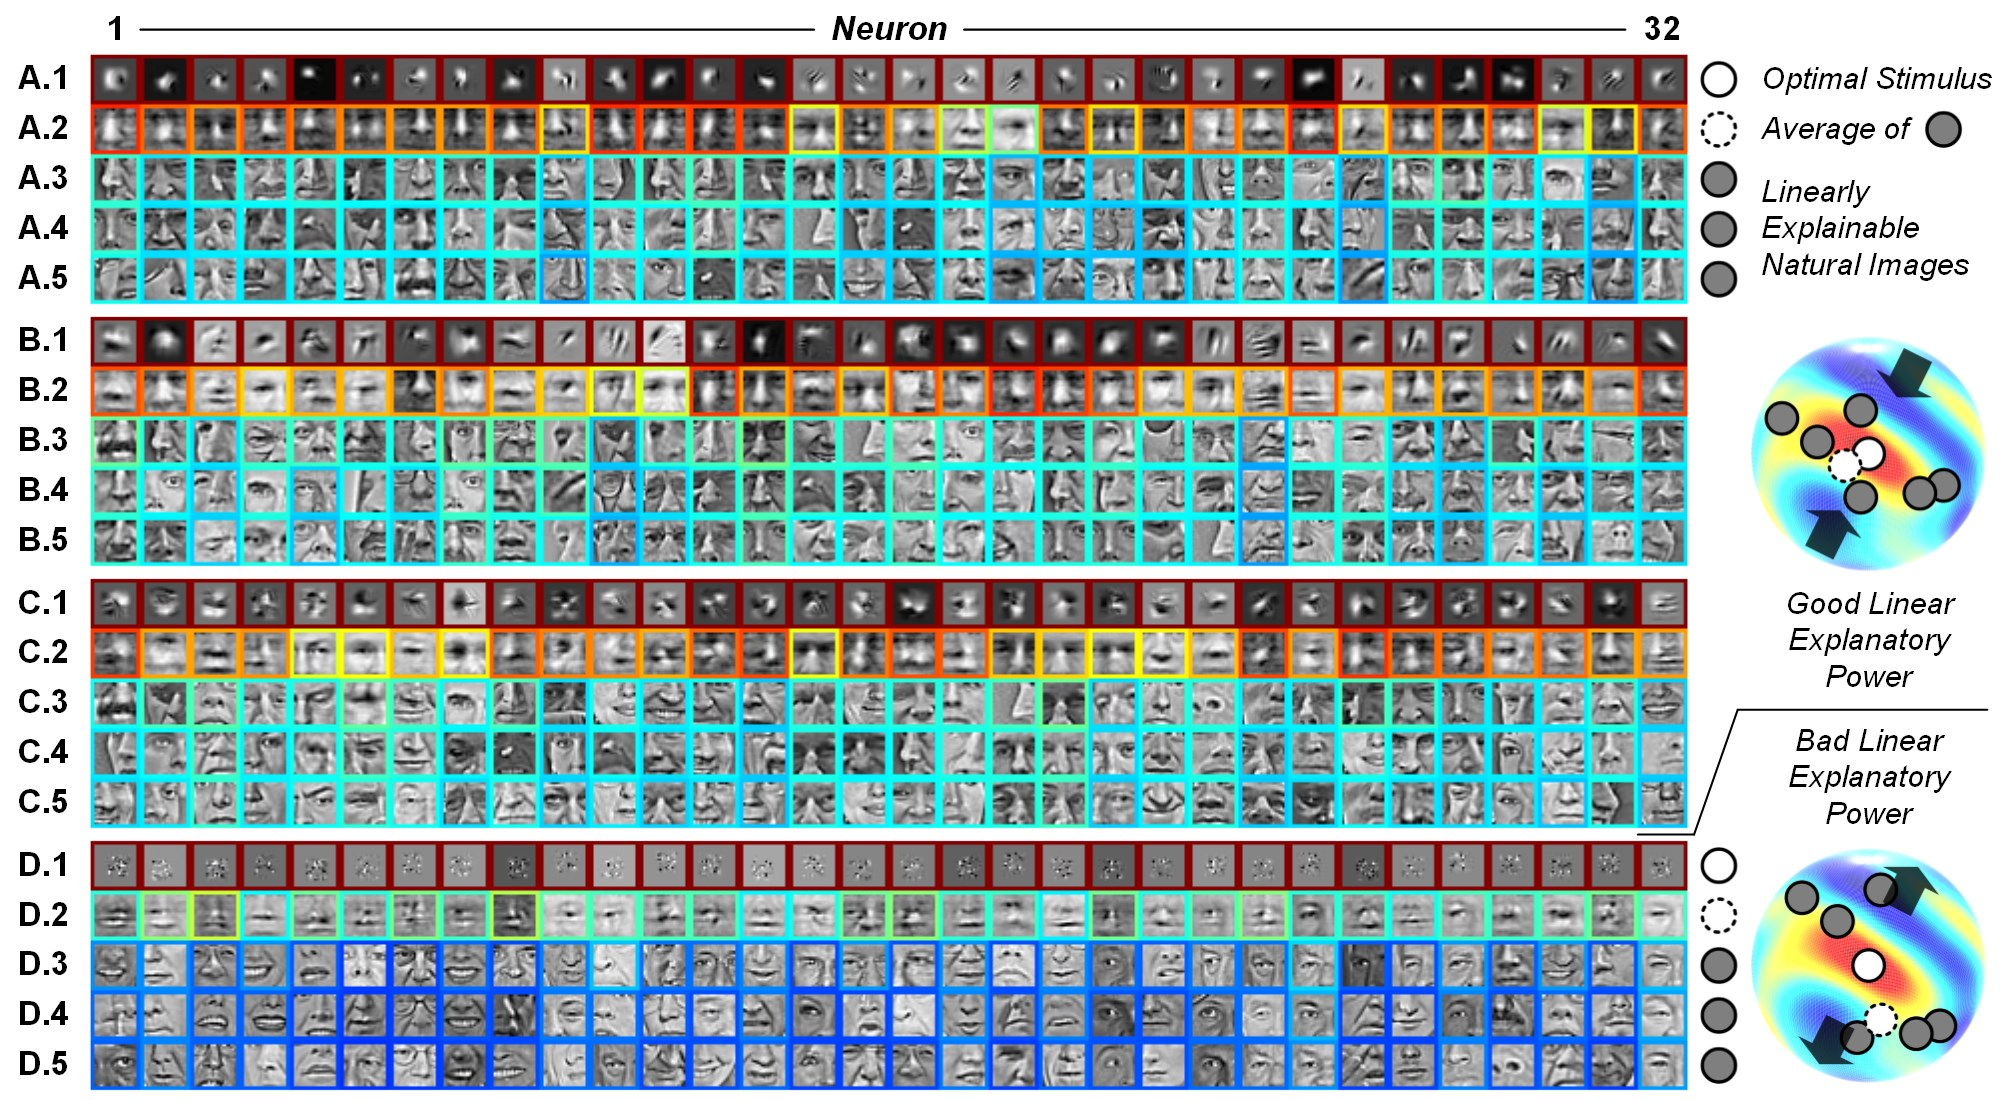
\includegraphics[width=0.85\textwidth]{Figs/pic2.jpg} 
\end{center}
\caption{{\bf Explanatory power of optimal stimuli of deep neurons.}
Results from deep networks of the top 3 strongest average explanatory power (A--C) and the weakest average explanatory power (D) are visualized.
Within each panel, the first row shows all 32 neurons' optimal stimuli from the network, the third to fifth rows show natural images with the top 3 strongest ``explainabilities'' (\ie inner-product distances between the images and the corresponding optimal stimuli), and the second row shows the average of images with top 100 explainabilities, out of 10,000 natural images.
Color of the boarder of an image indicates the explainability of the image, with color map following the definition in Fig.~\ref{fig:methods}.
Comparing deep networks' explanatory power and performances shows significant correlation (OSEP measure in Fig.~\ref{fig:corr}), which suggests \emph{``representing'' natural images can be required in first-order properties of good deep scalar representations (\ie optimal stimuli)}.
}
\label{fig:exppow}
\end{figure*}

\begin{figure}
\begin{center}
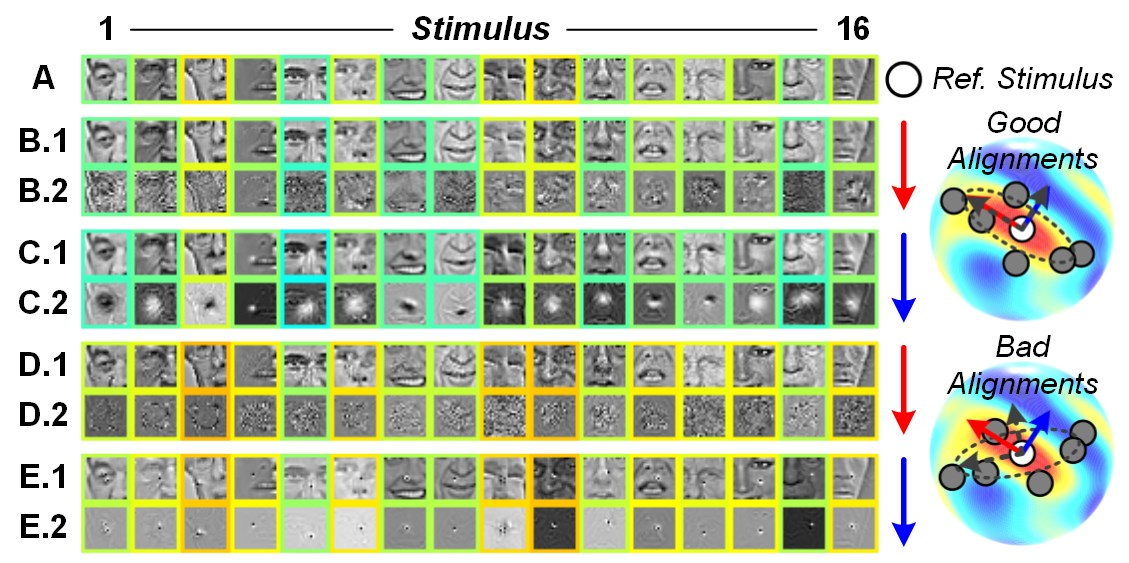
\includegraphics[width=\columnwidth, trim=1em 0 1em 0]{Figs/pic3.jpg} 
\end{center}
\caption{{\bf Alignments of subspaces between invariance and selectivity paths and natural images.}
Using 16 natural images in A as reference stimuli, the invariance paths with $\delta = 0.1\pi$ corresponding to the best alignments against natural images (\ie $L^1$ sparsities of images represented in eigenface coordinates) among all deep networks are shown in B.1, and similarly, worst alignments of invariance paths in C.1, best alignments of selectivity paths in D.1, and worst alignments of selectivity paths in E.1.
Differences between A and B.1--E.1 are shown in B.2--E.2 for clearer visualization.
Color of the boarder of an image indicates the alignment of the image against natural images, with color map following the definition in Fig.~\ref{fig:methods}.
As good alignments (B.1 and C.1) appear more natural (like structural deformations or lighting changes), bad alignments are mostly meaningless noises.
Comparing deep networks' subspace alignment measures and performances shows significant correlations (ITSA/STSA measures in Fig.~\ref{fig:corr}), which suggest \emph{a resemblance to natural image distributions can be required in second-order properties of good deep vector representations (\ie invariance and selectivity subspaces)}.
} %of subspaces % which are known to be important factors in visual recognition % accordingly
%Multiple runs of invariance and selectivity path searches are executed to form samples of the subspaces.
\label{fig:align}
\end{figure}

\begin{figure}
\begin{center}
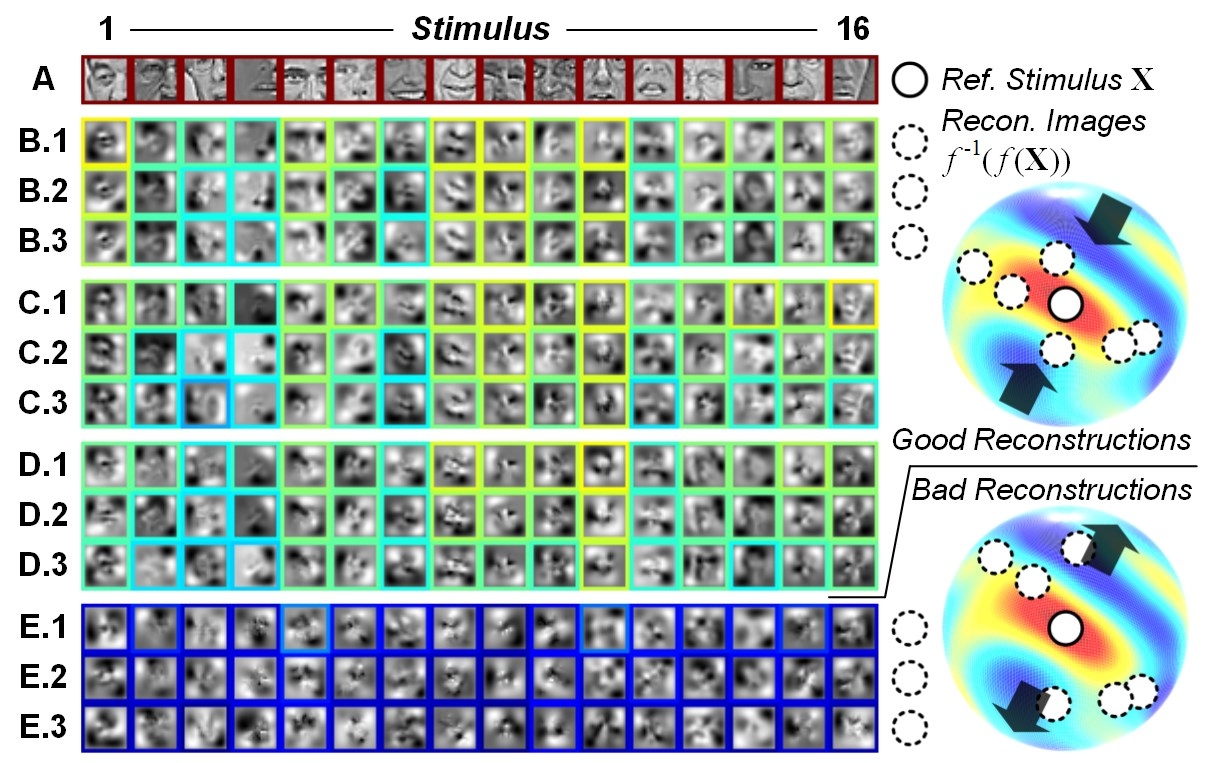
\includegraphics[width=\columnwidth, trim=1em 0 1em 0]{Figs/pic4.jpg} 
\end{center}
\caption{{\bf Reconstructability of deep vector representations (\ie encoding specificities of natural images).}
Using 16 natural images in A as reference stimuli, 3 examples of reconstructions from all deep networks with the best, second best, third best and worst average reconstructed image quality (SSIM) are shown in B--E respectively.
Color of the boarder of an image indicates the SSIM score between the image and reference stimulus, with color map following the definition in Fig.~\ref{fig:methods}.
Though the reconstructions are in general of lower spatial frequencies, some of the better ones do capture the spatial structures of reference stimuli decently well (\eg stimulus 1, 5, \etc).
Comparing deep networks' encoding specificities and performances shows significant correlations (ITSA/STSA measures in Fig.~\ref{fig:corr}), which suggest \emph{providing specific (\ie non-confounding) encoding of natural images can be required in first-order properties of good deep vector representations}.
} % (reconstructed)
\label{fig:encspc}
\end{figure}

\begin{figure}
\begin{center}
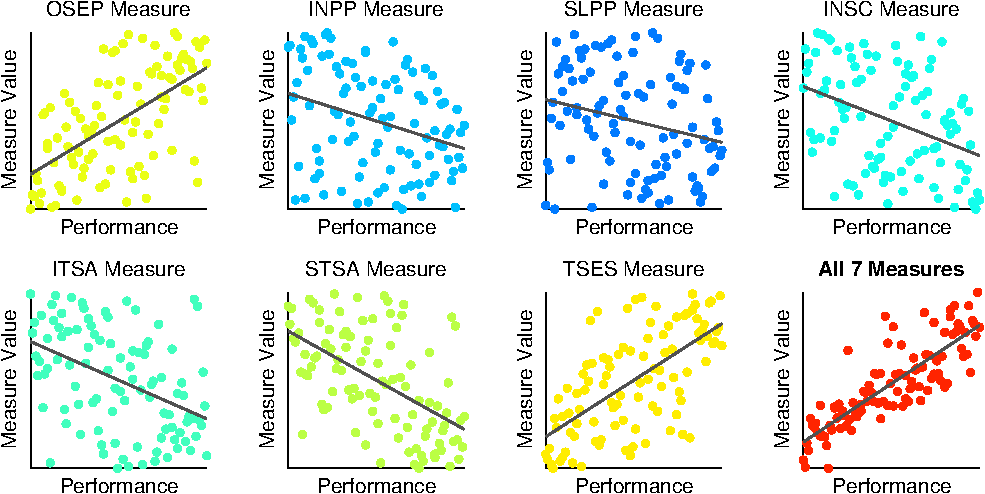
\includegraphics[width=0.95\columnwidth]{Figs/e_fig7_scatter-crop.pdf} 
\end{center}
\caption{{\bf Spearman's correlations between deep network's representation measures and performance.}
Representation measures following the raster order are, optimal stimulus explanatory power (OSEP), invariance path potential (INPP), selectivity path potential (SLPP), invariance subspace capacity (INSC), invariance \vs task-related image subspace alignment (ITSA), selectivity \vs task-related image subspace alignment (STSA), task-related image encoding specificity (TSES), and all 7 measures together using linear multiple correlation analysis.
Correlations $\rho$ and significance levels\footref{fnote:defstars} are $0.60^{\ast\ast\ast}$, $-0.31^{\ast\ast}$, $-0.24^{\ast}$, $-0.39^{\ast\ast\ast}$, $-0.44^{\ast\ast\ast}$, $-0.56^{\ast\ast\ast}$, $0.64^{\ast\ast\ast}$, and $0.84^{\ast\ast\ast}$, respectively.
Overall, \emph{71\% of the variance ($\rho^2$) of deep networks' performances can be explained} using the proposed representation measures altogether.
}
\label{fig:corr}
\end{figure}

{\bf Optimal stimulus explanatory power.} To understand how the optimal stimulus may affect a network's performance, we {tested} how well the optimal stimulus may ``linearly explain'' natural images and how the explanatory power correlates with a network's performance.
In total, 10,000 image patches {were} randomly cropped out of the predefined facial regions of pictures from the LFW-a dataset \cite{wolf2011effective} and compared against the optimal stimuli of all 32 top-layer neurons from all 100 deep networks. 
Figure \ref{fig:exppow} shows the results of best 3 and worst 1 networks in terms of explanatory power, which is estimated as the mean of the linear explainability of natural images, or inner-product distances between the optimal stimulus and $n$ nearest natural images $\left\lbrace {\bf{x}}^{t} \right\rbrace$, \ie $\frac{1}{n}\sum_{i=1}^{n} \langle {\bf{x}}^{t}_{i} , \hat{{\bf{x}}} \rangle$ with $n=100$, to measures how well the optimal stimulus can linearly ``approximate'' natural images (or intuitively how much neuronal response might be elicited).
It can be observed that, though none of the natural images is highly similar to any of the optimal stimuli, when alternatively comparing the averages of natural images of the top 1\% explainabilities and the optimal stimuli, the similarities (Fig.~\ref{fig:exppow}A.1 \vs \ref{fig:exppow}A.2, \etc) and dissimilarities (Fig.~\ref{fig:exppow}D.1 \vs \ref{fig:exppow}D.2) become apparent.
Such kind of ``linearities'' around task-related images out of the well-performing highly-nonlinear networks were observed in previous studies \cite{le2012building, simonyan2013deep} too, where optimal stimuli also resembled averages or combinations of visual objects.

%For simplicity and clarity of presentation, the explanation power measure is calculated using the top 1\% (i.e.~100) of the task-related stimuli with highest explainabilities, without biasing the results compared to using all task-related stimuli. 

{\bf Invariance and selectivity \vs natural image subspace alignment.} It has been shown that invariance and selectivity are extremely important for biological vision \cite{desimone1991face, ito1995size}; however, how these properties directly affect the recognition performance of artificial neural networks remains unclear.
To address this question, starting from 16 randomly sampled reference stimuli, invariance and selectivity path searches {were} performed at $\delta = 0.1\pi$ using Eq.~\ref{eq:I2}, \ref{eq:S2} for vector representations. 
Figure \ref{fig:align}B--E demonstrate the results of invariance and selectivity subspace alignment analyses, which measures the alignment between subspaces formed by natural images and invariance and selectivity paths (\ie how likely the invariance and selectivity can benefit recognition) via estimating the sparsity of $n$ paths projected onto the principal component vectors $\bf{V}$ of natural images $\left\lbrace {\bf{x}}^{t} \right\rbrace$, i.e.~$\frac{1}{n}\sum_{i=1}^{n} \left\| {\bf{Vx}}_{\delta,i} \right\|_{1}$ with $n=20$ and $\delta=0.1\pi$.

%quiroga2005invariant
%It can be observed that good alignments (\ie sparser representations in the principle component vector spaces) correspond to highly structural deformations or lighting changes, which are known to be important factors in visual recognition, while bad alignments correspond to mostly meaningless noises.

\newcommand{\expregular}{While Equation \ref{eq:O2} describes the essence of our approach, it was not able to produce analyzable numerical results alone, due to the fact that deep representations can be highly invariant to noises that do not resemble natural images.
Implementation-wise, it was further regularized with the energy of Laplacian filtering $\left\| \mathcal{L} \left( \bf{x} \right) \right\|$ to enforce smoothness and similarity to natural images.
A similar concept was also adopted in~\cite{mahendran2014understanding}.
}  %, with regularization constant decided via optimizing withheld data.

{\bf Encoding specificity of natural images.} To further understand the meaning of a vector representation $\bf{r}$ formed by a deep network $f$, the inverse function $f^{-1}\left( \bf{r} \right)$ {was} numerically approximated to reveal what kind of stimulus can drive the deep network to give output $\bf{r}$. 
Instead of inverting a randomly generated $\bf{r}$, which may not have feasible or interpretable solutions, we {used} $\bf{r}$ from a known reference stimulus $\tilde{\bf{x}}$ to study the encoding specificity and its relationship to performance.
Figure \ref{fig:encspc} shows the reference stimuli, the best 3 and worst 1 examples of encoding specificities, where the optimal stimulus search (Eq.~\ref{eq:O2}) is utilized as an inverse function of representations\footnote{\expregular}, and the average of structural similarities (SSIM) \cite{wang2004image} between the task-related reference stimulus $\tilde{\bf{x}}$ and $n$ reconstructed stimuli from random initializations, \ie $\frac{1}{n}\sum_{i=1}^{n} \mathrm{SSIM}\left(\tilde{\bf{x}} , \hat{{\bf{x}}}_i \right)$ with $n=10$, is measured to indicate how specific (or non-confounding) a representation is encoded.
While similar studies \cite{mahendran2014understanding, long2014convnets, razavian2014persistent} also employed such kind of ``reconstructability'' to study the representations of deep networks, our results suggest that, this property can actually be required for a deep network to perform well.

%SSIM measured using default settings of the standard implementation \cite{wang2004image} while different settings also yield similar correlations; other similarity measures like SNR, PSNR, and inner-product distance yield similar correlations as well

%Encoding specificity, as a single representation measure, can best explain the deep network's performance. Though bearing strong similarity to the invariance path search in terms of mathematical formulations, encoding specificity is in fact a radically different and complementary measure, since its numerical optimization is not constrained through distances to the reference stimulus (while distance constraints can induce \emph{a priori} similarities); thus, it can better function as an unconstrained global characterization of the ``encoding landscape'' (i.e.~multivariate tuning landscape of a population) and estimate if the (reconstructed) stimuli that a deep network is invariant to are ``selective'' (i.e.~visually similar to original stimuli). 

\newcommand{\defvecpp}{Since no baseline can be defined for vector representations likewise, the invariance (and selectivity, similarly) path potential is redefined as path integral on the fitness landscape $\int_{0}^{\frac{\pi}{2}}{\exp\left(-\left\|f\left(\bf{x}^{+}_{\delta}\right)-f\left(\hat{\bf{x}}\right)\right\|\right)}\mathrm{d}\delta \mathbin{/} {\frac{\pi}{2}}$.}

\newcommand{\expinsc}{Vector representation's INSC is negatively correlated to network's performance, mainly due to the fact that poorer performing network's invariance paths are usually noisier (as depicted in Fig.~\ref{fig:align}D), and thus should be interpreted differently from scalar representation's INSC.}

\newcommand{\expextrinsic}{As second-order properties, INPP, SLPP, and INSC are measures of search results \emph{started} from task-related images, but not \emph{ended} compared against them, unlike ITSA and STSA.
Task-unrelated measures, \ie OSSC, INPP, SLPP, and INSC of scalar representations as used in Fig.~\ref{fig:pair}, are significantly worse at explaining a network's performance (altogether with linear multiple correlation of only $0.34$), as one would expect.
}

{\bf Overall comparison.} Spearman's correlations between all representation measures and 100 deep networks' performances are summarized in Fig.~\ref{fig:corr}, and 71\% of the variance of deep networks' performances are explainable with the proposed measures altogether using linear multiple correlation analysis.
These measures further break down the differences among deep representations and suggest features like network's explanatory power, invariance and selectivity subspace properties, and encoding specificities against the task-related stimuli, can be extremely important for the effectiveness of representations.
Invariance and selectivity path potentials\footnote{\defvecpp} and invariance subspace capacity\footnote{\expinsc} for deep vector representations, on the other hand, have lower correlations to network's performance (though still significant), possibly due to their nature of being less task-related\footnote{\expextrinsic} than subspace alignment measures.
Worth to note, although the first-order properties (OSEP and TSES) have stronger individual correlations, they do not explain more about the network's performance than the other second-order properties, using linear multiple correlation analyses ($0.56$ \vs $0.58$).

%Network's invariance subspace capacity (in terms of population representation), which though has an $R^2=0.15$ correlation as well, is in fact negatively correlated to network's performance, mainly due to the fact that poor performing network's invariance path search results are usually noisier (as depicted in Fig.~\ref{fig:align}D), and thus should be interpreted differently from the unit representation cases. on the other hand, are weaker in explaining networks' performances (with $R^2=0.10/0.06$), due to the fact that all deep networks have high but less ranked invariance and selectivity.

\section{Discussion}

%how to intrepret results
{\bf Contributions of this work.} Comparatively, the characterization of representations in this work is designed to be general and unbiased such that both first- and second-order methods can be supported for single neurons or groups of neurons, without assuming any \emph{de facto} property in the solutions (\eg parametric deformations as used for studying invariance in previous works).
Additionally, with the strong statistical significances of results obtained from the large-scale experiments on 100 shallow and 100 deep networks, totalling 6,400 artificial neurons, we argue that our observations toward answering the differences between (shallow \vs deep) and among (deep) representations are highly conclusive, which can be summarized as:
\begin{itemize} % Main Findings
\setlength\itemsep{0.0ex}
\item Complexity of representations quantitatively increases along with network's depth.
\item Unlike a deep representation which is both invariant and selective, shallow representation is only invariant, not selective, and its capacity of invariance is significantly lower than a deep representation's.
\item Both first-order properties of deep representations (optimal stimulus explanatory power and encoding specificity of natural images) are crucially important to deep network performance.
\item All second-order properties of deep representations (in particular, invariance and selectivity \vs natural image subspace alignment) together are as important as first-order properties, if not significantly more.
\end{itemize}

{\bf Future work.} In this work, we only studied shallow networks and the ``simplest'' type of deep networks, two-level networks.
Although our results can potentially generalize if viewed as the characterization of ``adding an extra level'', it is still highly desirable to extend the study into deeper networks.
While the methods and measures proposed in this work are neutral to the depth of networks, numerical difficulties (\eg evaluation and convergence speed, quality of solutions, \etc) may need to be addressed in very deep networks.
Beyond explaining what properties make a deep representation good, it would be valuable too to incorporate these findings in learning even better representations, which are almost solely driven by bigger datasets nowadays, via certain kind of regularizations.  
We argue that this could be useful in accelerating or improving representation learning, especially when data are scarce and representations are not easily transferable.
Finally, even though a decently high fraction of the variance in deep networks' performances has been explained, how to further increase this number, if there is an upper bound (\eg limits from dataset itself), \etc, need to be further investigated.

%Secondly, statistical tests were extensively deployed to support observations reported in this paper, especially in the context of real applications (\ie LFW-a face recognition), which might seem still far-fetched to be fully explainable by mathematical theories.
%Nonetheless, we envision that combining more theoretical analyses which, \eg, have been adopted in various topics in understanding deep representations \cite{delalleau2011shallow, montufar2014number}, with statistical simulations can further empower us in answering other important questions in deep networks \cite{bengio2013deep}.

%%application
% application: where training data is scarse; actively regularize representations
% not deep in this work, but adding another layer(level), what would happen
% not only optimal stimulus; modulate the landscape
% theory works gave some general answers, we want to answer, in real apps, why.
% still, to combine with theory

%\clearpage

{\small
\bibliographystyle{ieee}
\bibliography{ref}
}

\end{document}
